\documentclass[
	german,
	accentcolor=10c,% Farbe für Hervorhebungen auf Basis der Deklarationen in den
	type=intern,
	marginpar=false
	]{tudapub}

\usepackage[english, main=german]{babel}
\usepackage[autostyle]{csquotes}
\usepackage{graphicx} % Required for inserting images
\setlength{\parskip}{1em}
\setlength{\parindent}{0pt}
\usepackage{subcaption}
\usepackage[backend=biber,style=numeric,sorting=none]{biblatex}  % oder style=numeric, authoryear etc.
\usepackage{minted}
\usepackage{amsmath}
\usepackage{float}
\usepackage[justification=centering]{caption}


\addbibresource{quellen.bib} 

%Formatierungen für Beispiele in diesem Dokument. Im Allgemeinen nicht notwendig!
\let\file\texttt
\let\code\texttt
\let\pck\textsf
\let\cls\textsf

\begin{document}


\title{Ultraschall zur Automatischen Erkennung Submentaler Muskeln und Bestimmung der Morphologie Mittels KI
}
\author{Malin Korner \& Carolina Halblaub}
%\date{} % Ohne Angabe wird automatisch das heutige Datum eingefügt

\maketitle


\section{Einleitung}
Der Begriff Dysphagie bezeichnet entweder Schwierigkeiten in den initialen Phasen des Schluckvorgangs oder das Gefühl, dass feste oder flüssige Nahrung auf dem Weg vom Mund in den Magen behindert wird. Insgesamt versteht man unter Dysphagie eine Störung beim Transport von geschluckten Substanzen \cite{ref1}.

Im klinischen Umfeld spielt die Dysphagie bei Patienten mit neurologischen Erkrankungen eine bedeutende Rolle und stellt eine häufige Komplikation nach einem Schlaganfall dar. Schätzungen zufolge entwickeln 25 bis 50 Prozent aller Schlaganfallpatienten eine Dysphagie. Diese kann zu Aspirationspneumonie, Mangelernährung und Dehydratation führen. Darüber hinaus beeinträchtigt Dysphagie die langfristige funktionelle Erholung und ist mit einer erhöhten Sterblichkeitsrate verbunden \cite{ref2}. Eine objektive Beurteilung der Dysphagie ist entscheidend für die Planung geeigneter Therapieansätze wie einer angepassten Diät oder der Verabreichung enteraler Ernährung \cite{ref3}.

Die in den Leitlinien empfohlenen diagnostischen Screening-Methoden, die videofluoroskopische Schluckuntersuchung (VFSS) und die fiberoptische endoskopische Evaluation des Schluckens (FEES), weisen jedoch Einschränkungen auf. Die FEES ist ein invasives Verfahren, dass nicht die orale Bolusvorbereitung oder den Zustand der Schluckmuskulatur einschätzen kann. Die VFSS gilt zwar als „Goldstandard“ zur Diagnostik der Dysphagie, ist jedoch mit Strahlenbelastung verbunden und erfordert in vielen Fällen den Transport von Schlaganfallpatienten, was die Anwendung unter bestimmten klinischen Bedingungen einschränkt \cite{ref2,ref3}. 

Ultraschall ist eine nicht-invasive und leicht zugängliche Methode, die auch zur Beurteilung des Schlucksvorgangs eingesetzt werden kann. In früheren Studien wurden verschiedene anatomische Referenzpunkte untersucht, darunter die Bewegung des Zungenbeins, eine verminderte Zungenbeweglichkeit oder die Hebung des Kehlkopfs. Die Ergebnisse blieben jedoch bislang inkonsistent \cite{ref2}.
Dies liegt vor allem daran, dass der Schluckvorgang ein hochkomplexer Prozess ist, der auf einer Vielzahl miteinander verbundener Funktionen basiert, darunter kognitive Prozesse, Bewusstsein, neuronale Bahnen und Muskelkraft. Eine Beeinträchtigung oder Veränderung eines dieser Faktoren kann die Schluckfunktion negativ beeinflussen, was die Entwicklung eines standardisierten Verfahrens zur Diagnostik der Dysphagie erschwert \cite{ref2,ref3}.

In den letzten Jahren hat die Anwendung von Künstlicher Intelligenz (KI) in der Medizin erheblich zugenommen \cite{ref3}. Dieser technologische Wandel hat Bereiche wie die fortschrittliche Diagnostik, die Behandlungsplanung, zielgerichtete Arzneimitteltherapien und chirurgische Verfahren maßgeblich beeinflusst. Eine treibende Kraft hinter diesen Fortschritten ist das Deep Learning (DL). DL ist ein Teilbereich des maschinellen Lernens, der auf neuronalen Netzwerken basiert und besonders präzise Vorhersagen ermöglicht \cite{ref4}.

Die Weiterentwicklung von DL-Techniken hat zur Integration von Objekterkennung und Bildsegmentierung geführt. Dadurch lassen sich spezifische Regionen innerhalb eines Bildes identifizieren \cite{ref3,ref4}. In der Medizin wurden DL-basierte Modelle erfolgreich eingesetzt, um Tumoren in Röntgenaufnahmen des Brustkorbs, CT-Scans und MRT-Bildern zu erkennen. Diese Modelle haben sich als effizient und zuverlässig erwiesen, insbesondere bei der Analyse medizinischer Bilddaten zur Bewältigung diagnostischer Herausforderungen \cite{ref3}.
Derzeit gibt es mehrere kommerziell erhältliche KI-Modelle, die physiologische Phänomene wie die Herzbewegung, den Blutfluss, die Komprimierbarkeit der Venen und die Bewegung der Vena cava inferior analysieren \cite{ref3,ref4}. Obwohl zahlreiche Studien KI-basierte Ansätze untersucht haben, um die diagnostische und therapeutische Genauigkeit bei Patienten mit Dysphagie zu verbessern, bleibt ihre Integration in die klinische Praxis bislang begrenzt \cite{ref4}.

Dies liegt unter anderem daran, dass die Ultraschalluntersuchung zwar als eine zugänglichere und kostengünstigere Methode zur Ermittlung relevanter physiologischer Parameter gilt, jedoch im Vergleich zur Computertomographie (CT) oder Magnetresonanztomographie (MRT) weiterhin erhebliche Einschränkungen aufweist. Dazu gehören insbesondere die inter- und intraindividuelle Variabilität bei der Durchführung der Ultraschalluntersuchungen und daraus resultierende nicht immer gut vergleichbare Bildqualität. Letztere erschwert die Reproduzierbarkeit und Konsistenz der Auswertung [5].Daraus ergibt sich ein dringender Bedarf an automatisierten Methoden, die auf DL basieren und eine standardisierte, objektive Analyse ermöglichen.

Das Hauptziel dieser Arbeit besteht darin, einen Beitrag zur Entwicklung eines solchen Modells zu leisten und somit langfristig zur Etablierung eines standardisierten diagnostischen Verfahrens beizutragen. In der ersten Phase der Entwicklungspipeline, die im Rahmen dieser Arbeit eingeleitet wurde, sind unter anderem die Datenerhebung, das Modelltraining und die erste Implementierung des Systems vorgesehen.

\section{Grundlagen}

\subsection{Physiologie des Schluckvorgangs}
Der Schluckvorgang ein komplexer Prozess, an dem viele Muskeln beteiligt sind. Wir haben uns in dem folgenden Projekt auf zwei beteiligte Muskelpaare fokussiert, da diese im Ultraschall gut zu erkennen sind. In Abbildung~\ref{fig:digastric-muscle} sieht man den rechten M. Digastricus, welcher Schläfenbein (Os temporale) und Unterkiefer (Mandibula) miteinander verbindet. Die Zwischensehne des Muskels ist durch ein ringförmiges Band am Zungenbein fixiert \cite{digastricus_explain}. 
Der M. Geniohyoideus, in Abbildung~\ref{fig:Geniohyoid-chin}, verbindet Zungenbeinkörper (Os hyoideum) mit Unterkiefer (Mandibula). Beim Schlucken heben diese Muskeln das Zungenbein an, welches wiederum zu einem Anheben von Zunge und Kehlkopf führt. Dadurch verschließt die Epiglottis (Kehldeckel) die Luftröhre und die Nahrung gelangt in die Speiseröhre.  
So wird verhindert, dass Nahrung in die Luftröhre gelangt \cite{geniohyoideus_explain,digastricus_explain}.

\begin{figure}[h]
    \centering
    \begin{subfigure}[b]{0.3\textwidth}
        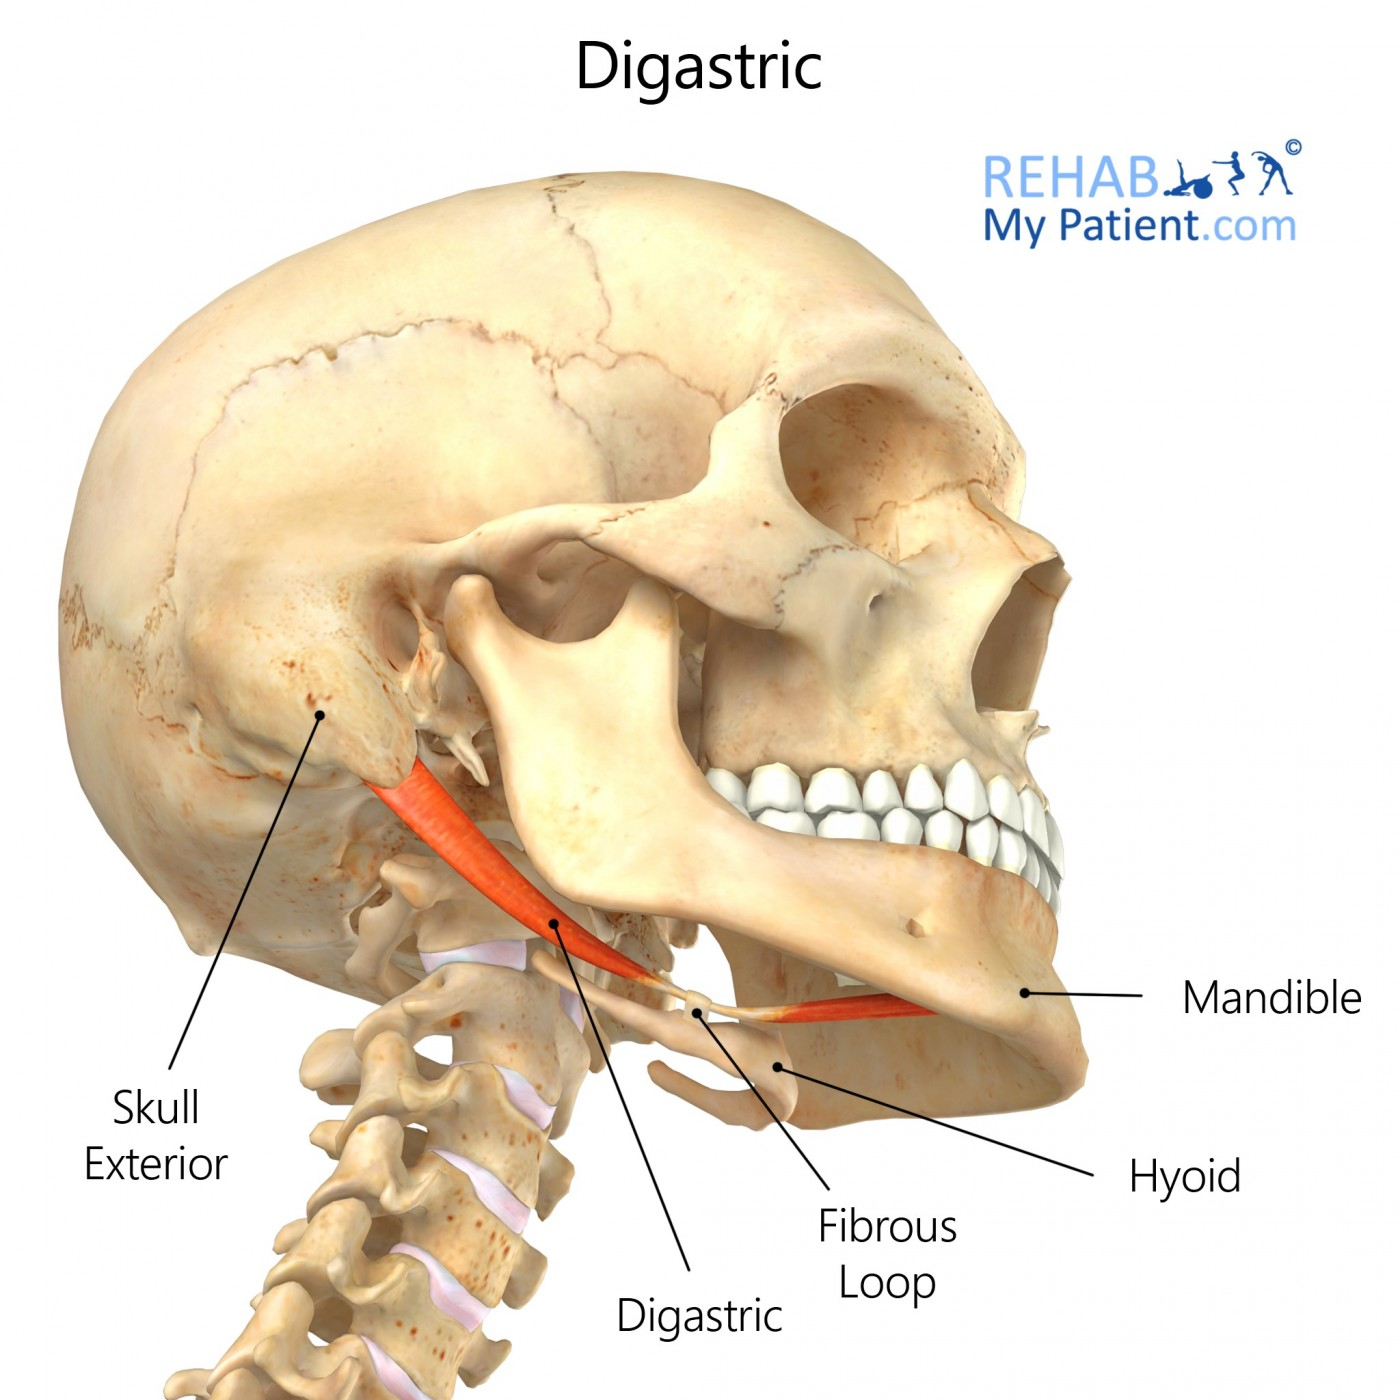
\includegraphics[width=\textwidth]{digastric-muscle}
        \caption{M. Digastricus verbindet Schläfen-, Zungenbein und Unterkiefer \cite{digastricus}.}
        \label{fig:digastric-muscle}
    \end{subfigure}
    \hfill
    \begin{subfigure}[b]{0.3\textwidth}
        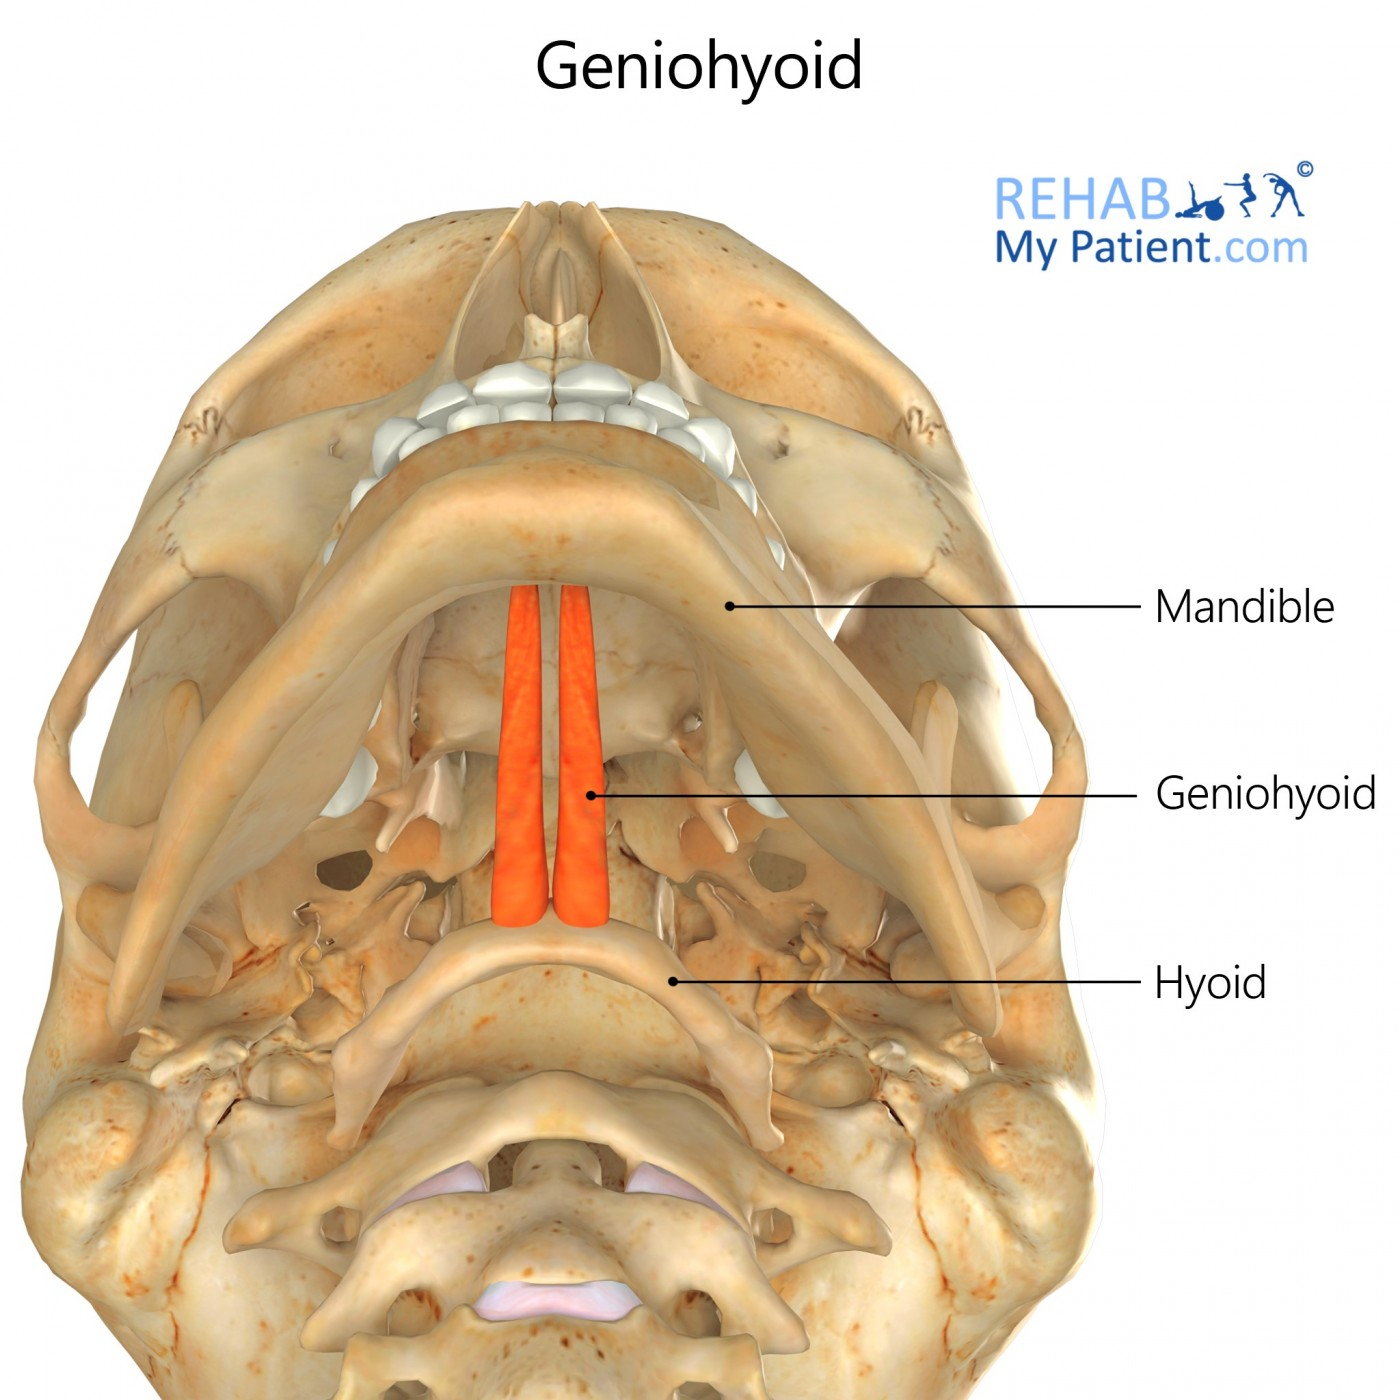
\includegraphics[width=\textwidth]{Geniohyoid-chin}
        \caption{M. Geniohyoideus verbindet Zungenbein mit Unterkiefer \cite{geniohyoideus}.}
        \label{fig:Geniohyoid-chin}
    \end{subfigure}
    \caption{Diese zwei Muskelpaare wurden in dem Projekt genauer betrachtet.}
    \label{fig:muskeln}
\end{figure}

\subsubsection{Dysphagie}
Der Begriff Dysphagie stammt aus dem Griechischen und setzt sich aus "dys" (= erschwert, gestört) und "phagein" (= essen) zusammen. Er bezeichnet eine Beeinträchtigung des Schluckvorgangs von fester Nahrung und Flüssigkeiten. Je nach Ausprägung kann diese Schluckstörung die Nahrungsaufnahme deutlich erschweren oder sogar vollständig verhindern, sodass Nahrung und Flüssigkeit nicht mehr in die Speiseröhre und den Magen gelangen.

Schluckstörungen können zu erheblichen körperlichen Folgen wie Mangelernährung und Dehydrierung führen und das Mortalitätsrisiko erhöhen. Daher ist es entscheidend, eine Dysphagie frühzeitig zu erkennen, um eine adäquate Therapie einzuleiten und die Ernährung anzupassen \cite{ref6}.

\subsection{Künstliche Intelligenz in der Medizin}

In den letzten Jahren hat die Medizin eine Phase tiefgreifender Veränderungen durchlaufen, die maßgeblich durch Fortschritte in der medizinischen Informatik vorangetrieben wurden \cite{ref9}. Im Jahr 2017 genehmigte die U.S. Food and Drug Administration (FDA) die erste Software für die kardiale Magnetresonanztomographie, die auf künstlicher Intelligenz (KI) basierte. Sie trug den Namen Cardio AI und ebnete damit den Weg für viele weitere KI-gestützte Produkte, die ebenfalls eine behördliche Zulassung erhielten. Dies hat die Forschung und Innovation in diesem Bereich weiter beschleunigt \cite{ref11}. Zu den bemerkenswerten Entwicklungen zählen modernste Diagnoseverfahren, fortschrittliche Behandlungsmethoden, gezielte Arzneimitteltherapien und innovative chirurgische Techniken, die zunehmend durch KI-Technologien unterstützt werden \cite{ref9}.

Maschinelles Lernen (ML), ein Teilbereich der KI, bei dem Algorithmen eingesetzt werden, um mit hoher Genauigkeit Ergebnisse vorherzusagen, ist eines der bedeutendsten Anwendungsfelder der KI in der Medizin. Innerhalb des maschinellen Lernens ist das Deep Learning (DL) ein Teilgebiet, das vor allem neuronale Netzwerke nutzt, um eine noch höhere Vorhersagegenauigkeit zu erreichen. In der Medizin werden DL-basierte Algorithmen wegen ihrer Effizienz und Robustheit geschätzt. Sie werden am häufigsten in der medizinischen Bildgebung eingesetzt, um diagnostische Herausforderungen zu bewältigen \cite{ref9}. Deep-Learning-Modelle, insbesondere Convolutional Neural Networks (CNNs), verarbeiten medizinische Bilder in aufeinanderfolgenden Schichten, die zunehmend komplexere Muster erkennen. Frühere Schichten erfassen grundlegende visuelle Elemente wie Kanten, Texturen und einfache Formen, während tiefere Schichten diese zu höherstufigen Merkmalen kombinieren, die anatomische Strukturen oder pathologische Regionen darstellen \cite{ref11}.

Solche Fortschritte haben in der medizinischen Bildgebung neue Möglichkeiten für die Segmentierung und Quantifizierung eröffnet. Mithilfe gut trainierter Modelle können KI-Systeme Strukturen von Interesse in medizinischen Bildern, wie Tumoren, Blutgefäße oder Zellen, präzise abgrenzen. Diese Segmentierungsfähigkeit ermöglicht eine schnelle und präzise Verarbeitung der Bilder und ist von unschätzbarem Wert für die Erkennung von Krankheiten im Frühstadium und die Behandlungsplanung. Ärztinnen und Ärzte können damit Anomalien identifizieren, die mit herkömmlichen Diagnosemethoden möglicherweise übersehen würden. Sie können gezielt Interventionsbereiche festlegen, chirurgische Eingriffe optimieren und gezielte Therapien durchführen \cite{ref9,ref11}.


\subsubsection{Bild Segmentierung}

Die Bildsegmentierung ist ein entscheidender Schritt in der medizinischen Bildgebung und bildet die Grundlage für präzise Diagnosen, Behandlungspläne und quantitative Analysen in einer Vielzahl klinischer Anwendungen. Dabei wird ein Bild in klar abgegrenzte Regionen unterteilt, wie anatomische Strukturen oder pathologische Bereiche. Zum Beispiel Organe, Gewebe oder Läsionen. Dies wird auch Region of Interest bezeichnet (ROI). Dies ermöglicht eine präzise Interpretation medizinischer Bilder und unterstützt wesentliche Aufgaben, wie die Lokalisierung von Tumoren, die Abgrenzung von Organrändern und die präoperative Planung.

Je nach Komplexität der ROI und der umliegenden anatomischen Strukturen kann die Annotation eines einzelnen Bildes jedoch mehrere Minuten bis hin zu mehreren Stunden in Anspruch nehmen. In praktischen Anwendungen des Deep Learning ist ein gewisses Maß an Label-Rauschen unvermeidlich und für die Erstellung zuverlässiger Annotationen ist häufig die Übereinstimmung von mehr als drei Fachexpert:innen erforderlich. Vorhandene Verzerrungen in den annotierten Daten können sich auf die trainierten Modelle übertragen und deren Leistung potenziell beeinträchtigen. Folglich bleibt die Bildsegmentierung eine zeitaufwändige und komplexe Aufgabe, deren Genauigkeit sich direkt auf die klinischen Ergebnisse auswirkt und die somit eine unverzichtbare Komponente moderner Gesundheitssysteme darstellt \cite{ref10}.

\subsubsection{Data Augmentation}
Bilder manuell zu segmentieren, ist sehr zeitaufwendig. Insgesamt ist ein Datensatz von 300 Bildern noch sehr wenig. Um möglichst schnell einen größeren Datensatz zu erreichen, wird im folgenden Augmentation verwendet. Das bedeutet, dass vorhandene segmentierte Bilder leicht verändert werden. Die Bilder werden zum Beispiel gespiegelt, gedreht oder die Helligkeit und die Sättigung wird verändert, wie in Abbildung~\ref{fig:Augmentation} zu sehen. Dies führt insgesamt zu einem robusteren System, einer Reduktion von Overfitting und einer höheren Generalisierbarkeit des trainierten Modells \cite{Augmentation}.

\begin{figure}[H]
    \centering
    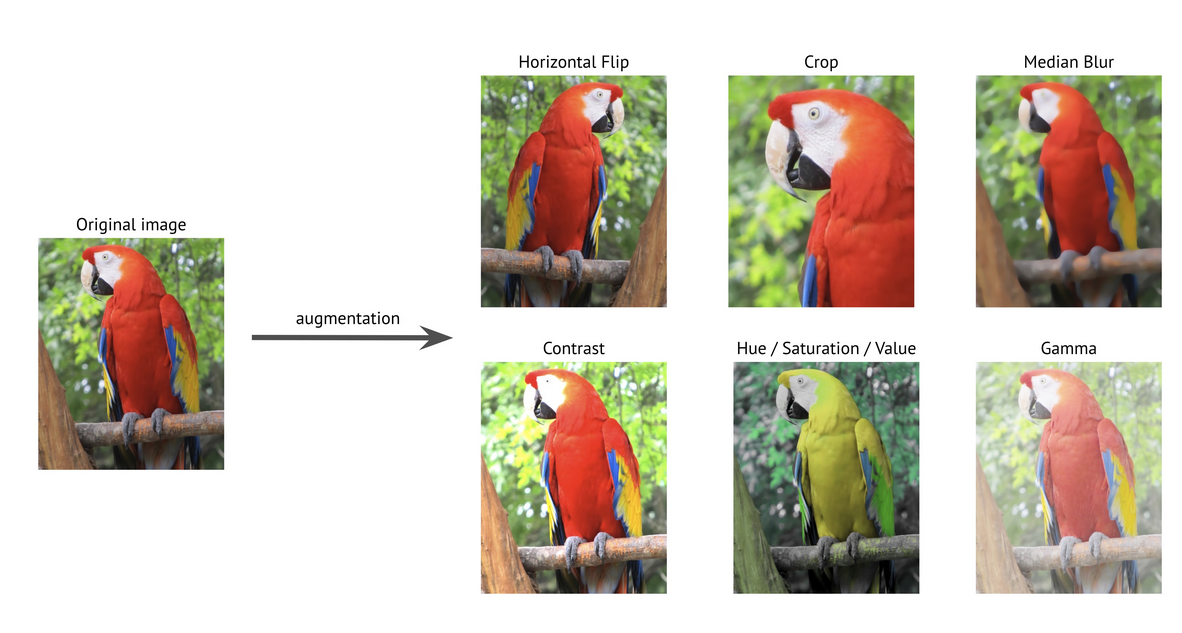
\includegraphics[width=0.6\textwidth]{Augmentation.png}
    \caption{Mögliche Augmentation eines Bildes \cite{Augmentation}.}
    \label{fig:Augmentation}
\end{figure}

\subsubsection{YOLO und CVAT}
YOLO (You Only Look Once) ist ein Echtzeit-Bildsegmentierungs- und Objekterkennungsmodell. Dieses basiert auf einem Convolutional Neural Network. 2015 wurde YOLO auf den Markt gebracht und von Joseph Redmon und Ali Farhadi an der University of Washington entwickelt. Seitdem gibt es immer wieder verbesserte neuere Versionen von YOLO. Seit 2024 gibt es die momentan aktuellste Version YOLOv11, welche in unserem Projekt verwendet wurde. Für verschiedene Computer-Vision-Aufgaben gibt es bestimmte Modelle. Im folgenden wurde YOLO11-seg verwendet, da dieses speziell für die Segmentierung entwickelt wurde. Desweiteren gibt es unterschiedliche Modellgrößen von YOLO. Es gibt nano, small, medium, large und extra large. In dem Projekt wird ein kleiner Datensatz von 300 Bildern verwendet. Kleine Modelle haben weniger Parameter und lernen dadurch nicht so schnell kleine Details, wie zum Beispiel Rauschen, bei kleinen Datensätzen. Große Modelle würden sich in diesem Fall schnell zu stark anpassen und sich die Trainingsdaten merken, anstatt zu generalisieren (Overfitting). Aus diesem Grund wurde die nano Version, YOLO11n-seg verwendet \cite{YOLO11}.


Das Computer Vision Annotation Tool (CVAT) ist eine leistungsstarke Plattform zur effizienten und präzisen Annotation visueller Daten. Es wurde entwickelt, um dem steigenden Bedarf an schnellen und zuverlässigen Werkzeugen zur Datenkennzeichnung gerecht zu werden, und ermöglicht die Erstellung hochwertiger, annotierter Datensätze für das Training von Deep-Learning-Modellen in verschiedenen Aufgaben der Computer Vision. 

Ein Beispiel hierfür ist die semantische Segmentierung, bei der mithilfe von Deep-Learning-Algorithmen jedem Pixel eines Bildes eine Klassenbezeichnung zugewiesen wird. Dadurch wird das Bild in unterschiedliche Regionen unterteilt, die jeweils einer bestimmten Kategorie zugeordnet sind. Diese feinkörnige Analyse ist insbesondere in der medizinischen Bildgebung von großer Bedeutung, da dort eine exakte Annotation entscheidend ist. CVAT hat sich dabei als besonders geeignet für medizinische Annotationen erwiesen, da es eine überzeugende Kombination aus Flexibilität, Skalierbarkeit und Kosteneffizienz bietet. Somit stellt es eine bevorzugte Lösung für KI-gestützte Anwendungen im Gesundheitswesen dar \cite{CVAT}.

\subsubsection{Performance Metriken in der KI}
Mit der zunehmenden Verbreitung und Relevanz von KI-Modellen in der Medizin ist es entscheidend, deren sicheren und effektiven Einsatz durch rigorose, verlässliche und kontextsensitiv angepasste Evaluierungen sicherzustellen.
Derzeit wird die Leistungsfähigkeit von KI-Modellen überwiegend anhand quantitativer Metriken bewertet, die Aufschluss über deren Eigenschaften und Performance geben. Trotz der Fortschritte in diesem Bereich bleibt das vollständige Verständnis der Funktionsweise eines Modells und dessen korrekte Evaluierung äußerst komplex \cite{ref7,ref8} . Daher muss auch das Einsatzszenario sorgfältig berücksichtigt werden. Bei Detektionsaufgaben in der medizinischen Bildgebung, wie beispielsweise der Identifizierung anatomischer Strukturen, sind spezielle Metriken erforderlich. Im Gegensatz zu einfacheren Klassifikationsaufgaben umfasst die Detektion nicht nur die Bestimmung der Anwesenheit eines Objekts, sondern auch dessen Position, die häufig durch sogenannte „Bounding boxen“ angegeben wird \cite{ref7}.

Im Rahmen dieses Projekts wurden die folgenden Metriken zur Bewertung der entwickelten Modelle gewählt:

Intersection over Union (IoU): In der Objekterkennung gibt der IoU-Wert das Ausmaß der Überlappung zwischen einer vorhergesagten Bounding Box und einer Referenz-Bounding Box (Ground Truth) an. Da es sich bei diesem Projekt um eine Bildsegmentierung handelt, werden nicht die Bounding Boxen sondern die Segmentierungsmasken des Modells verglichen. Der IoU wird wie folgt berechnet:
\[
IoU = \frac{\text{Fläche der Überlappung}}{\text{Fläche der Vereinigung}}
\]
Eine Vorhersage wird in der Regel als „True Positive” gewertet, wenn ihr IoU-Wert mit einer „Ground-Truth”-Box einen vordefinierten Schwellenwert überschreitet und sie korrekt zu diesem „Ground Truth” zugeordnet ist.

Recall: Recall misst den Anteil der tatsächlich positiven Beispiele, die korrekt erkannt werden, und wird wie folgt berechnet:

\[
Recall = \frac{\text{True Positives (TP)}}{\text{True Positives (TP)} + \text{False Negatives (FN)}}
\]

Recall ist besonders in medizinischen Studien von Bedeutung, da das Ziel darin besteht, so wenige positive Instanzen wie möglich zu übersehen.

Präzision: Die Präzision misst den Anteil der vom Modell als positiv vorhergesagten Instanzen, die tatsächlich korrekt sind, und wird wie folgt berechnet:

\[
Precision = \frac{\text{True Positives (TP)}}{\text{True Positives (TP)} + \text{False Positives (FP)}}
\]

Mean Average Precision (mAP): Die mAP ist der Mittelwert der Average Precision (Fläche unter der Präzisions-Recall-Kurve) über alle Objektklassen oder IoU-Schwellenwerte (0,5 - 0,95) und spiegelt sowohl die Präzision als auch die Genauigkeit der Lokalisierung wider \cite{ref7}.

\section{Methodik}
Um ein KI-gestütztes Modell zu entwickeln, das die Morphologie der submentalen Muskeln erkennen und bestimmen kann, wurden wie in Abbildung~\ref{fig:workflow} zu sehen, die folgenden Schritte durchgeführt. Die Datenerfassung, Datenvorverarbeitung, Bildsegmentierung von submentalen Ultraschallaufnahmen, Export der annotierten Daten im YOLO-Format, Erstellung verschiedener KI-Modelle und Leistungsbewertung und Vergleich der KI-Modelle.

\begin{figure}[H]
    \centering
    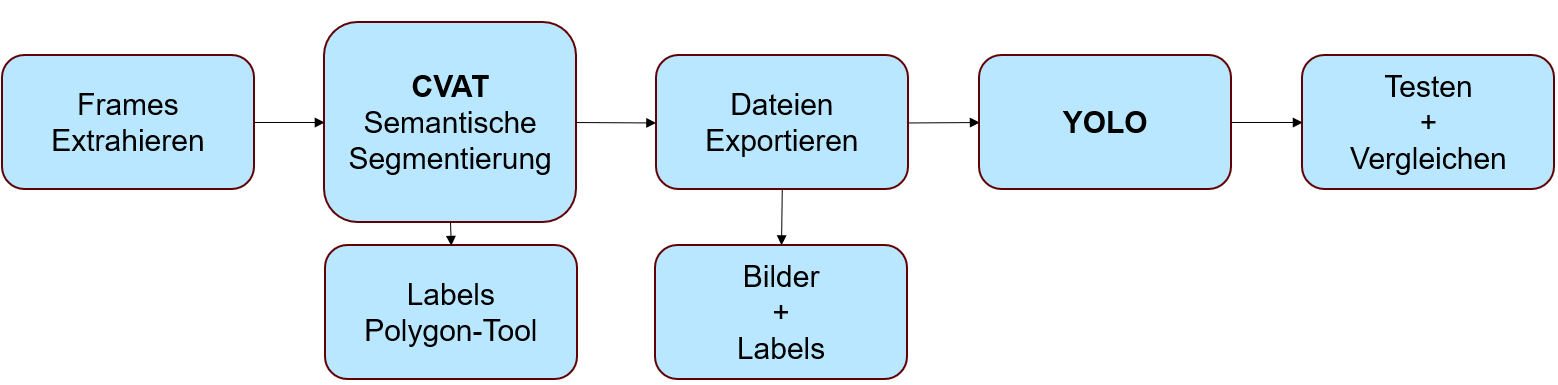
\includegraphics[width=0.7\textwidth]{workflow.png}
    \caption{Ablauf für die Entwicklung eines KI-gestützten Modells.}
    \label{fig:workflow}
\end{figure}

\subsection{Datenerfassung}
Zur Datenerfassung wurde der Schluckvorgang von insgesamt 15 gesunden Versuchspersonen im Klinikum Darmstadt mithilfe des Ultraschallgeräts Clarius Linearsonde 15 MHz untersucht. Darunter sind 6 Frauen und 7 Männer im Alter von 24 bis 36 Jahren. Von jeder Person wurden 10-sekündige Videos des Schluckvorgangs aufgenommen. Pro Person erfolgten zehn Aufnahmen beim Trockenschlucken sowie beim Schlucken von Wasser und Pudding. Dadurch entstanden 30 Videos pro Person und insgesamt 450 Videos.

\begin{figure}[H]
    \centering
    \includegraphics[width=0.6\textwidth]{versuchsdurchführung}
    \caption{Versuchsdurchführung.}
    \label{fig:versuchsdurchführung}
\end{figure}

Abbildung~\ref{fig:transversalMundboden} zeigt die Position des Ultraschallgeräts. Dabei wird die Sonde transversal auf den Mundboden aufgesetzt. 

\begin{figure}[H]
    \centering
    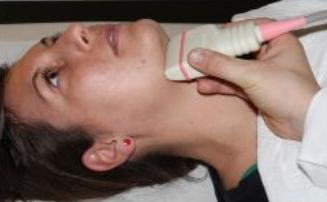
\includegraphics[width=0.3\textwidth]{transversalMundboden}
    \caption{Lage des Ultraschallkopfes \cite{mundboden}.}
    \label{fig:transversalMundboden}
\end{figure}

\subsection{Datenvorverarbeitung und Bildsegmentierung}
Da das Ziel der Ultraschallaufnahmen die semantische Segmentierung der einzelnen Videos war, wurden zunächst aus jedem Video 20 gleichmäßig verteilte Einzelbilder (Frames) extrahiert. Anschließend erfolgte mithilfe der Software CVAT die manuelle Segmentierung der relevanten Muskulatur. In der Abbildung~\ref{fig:Ultraschall_mit_Segmentierung} sieht man die Ultraschallaufnahmen mit den segmentierten Muskeln. Die drei markierten Bereiche können aufgrund ihrer Form leicht als „Mickey-Mouse-Struktur“ identifiziert werden. Links ist der Ruhezustand einer Person zu sehen, rechts der Moment des Schluckens. Dabei ist eine Veränderung der Muskulatur erkennbar, da sich Größe und Form der Muskeln verändern. Insgesamt wurden im Rahmen des Projekts 300 Bilder der Muskeln Musculus digastricus und Musculus geniohyoideus segmentiert. 

\begin{figure}[H]
    \centering
    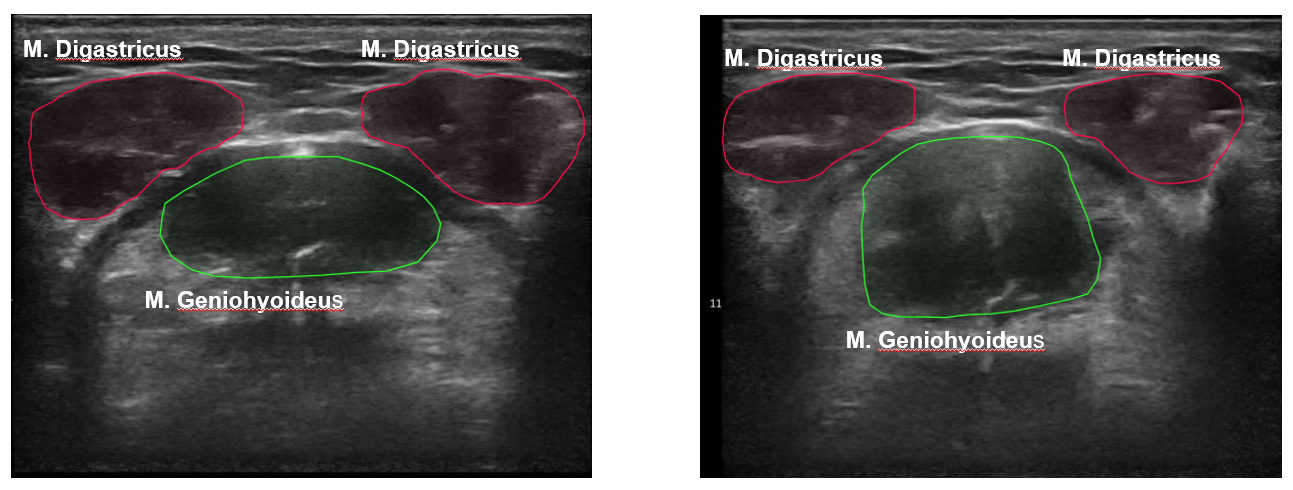
\includegraphics[width=0.5\textwidth]{Ultraschall_mit_Segmentierung}
    \caption{Ultraschallbild mit segmentierten Muskeln. Links ist der Ruhezustand und rechts schluckt gerade die Person.}
    \label{fig:Ultraschall_mit_Segmentierung}
\end{figure}

\subsection{Erstellung verschiedene KI-Modelle}
Nachdem die 300 Bilder vollständig segmentiert worden waren, wurden sie im Ultralytics-Format exportiert. Das bedeutet, dass die Daten in ein mit YOLO kompatibles Format umgewandelt wurden, das aus Bilddateien und den zugehörigen Label-Dateien im Textformat besteht.

Wie in Abbildung ~\ref{fig:datensatz} dargestellt, wurde der Datensatz in Trainings-, Validierungs- und Testdaten aufgeteilt. Der Trainingsdatensatz umfasst 210 Bilder (70\%), während der Validierungs- und der Testdatensatz jeweils 45 Bilder (15\%) enthalten. Da die Bilder von einer Person immer sehr ähnlich sind und sich nur in der Perspektive durch die Position des Ultraschallgerätes etwas unterscheiden, wurde der Datensatz nach den Personen aufgeteilt. Eine Person ist somit jeweils nur im Trainings-, Validierungs- oder Testdatensatz vorhanden. Sonst könnte sich das Modell zum Beispiel bestimmte Merkmale einer bestimmten Person lernen, welche nicht für ein generalisierbares Modell spricht. Durch die Aufteilung wird eine realistische Modellbewertung erreicht, da das Modell mit unbekannten Personen getestet wird.

\begin{figure}[H]
    \centering
    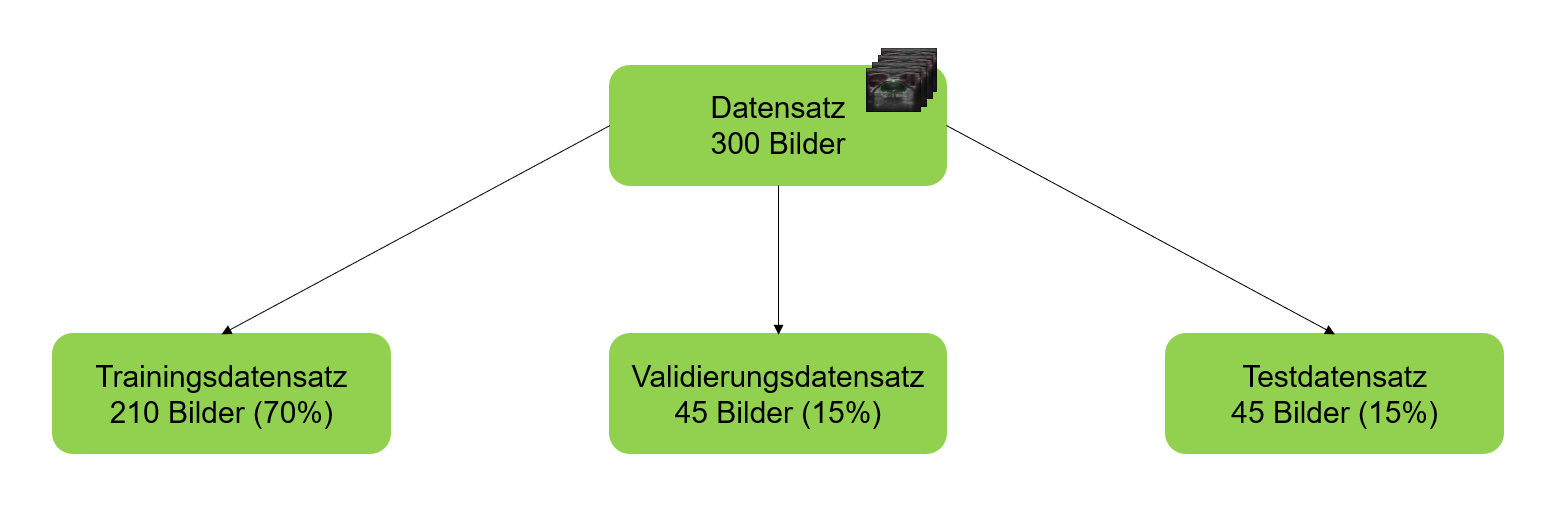
\includegraphics[width=0.6\textwidth]{Datensatz.png}
    \caption{Aufteilung des Datensatzes.}
    \label{fig:datensatz}
\end{figure}

Die Implementierung der Modelle erfolgte in der Programmiersprache Python innerhalb der Umgebung Google Colab. Zunächst war es notwendig, die Bibliothek Ultralytics zu importieren und das gewünschte YOLO-Modell, beispielsweise ein bereits vortrainiertes Modell wie YOLOv11, zu laden. Die Architektur von YOLOv11 ist in Abbildung~\ref{fig:YOLO_Architecture} zu sehen. Das Backbone extrahiert wichtige Merkmale aus dem Eingabebild. Danach werden diese Merkmale im Neck kombiniert, sodass feine und grobe Strukturen erfasst werden. Der Head erzeugt daraus die finale Vorhersage \cite{Rao2024Oct}. In diesem Projekt entspricht dies der Maske der erkannten Muskeln.

\begin{figure}[H]
    \centering
    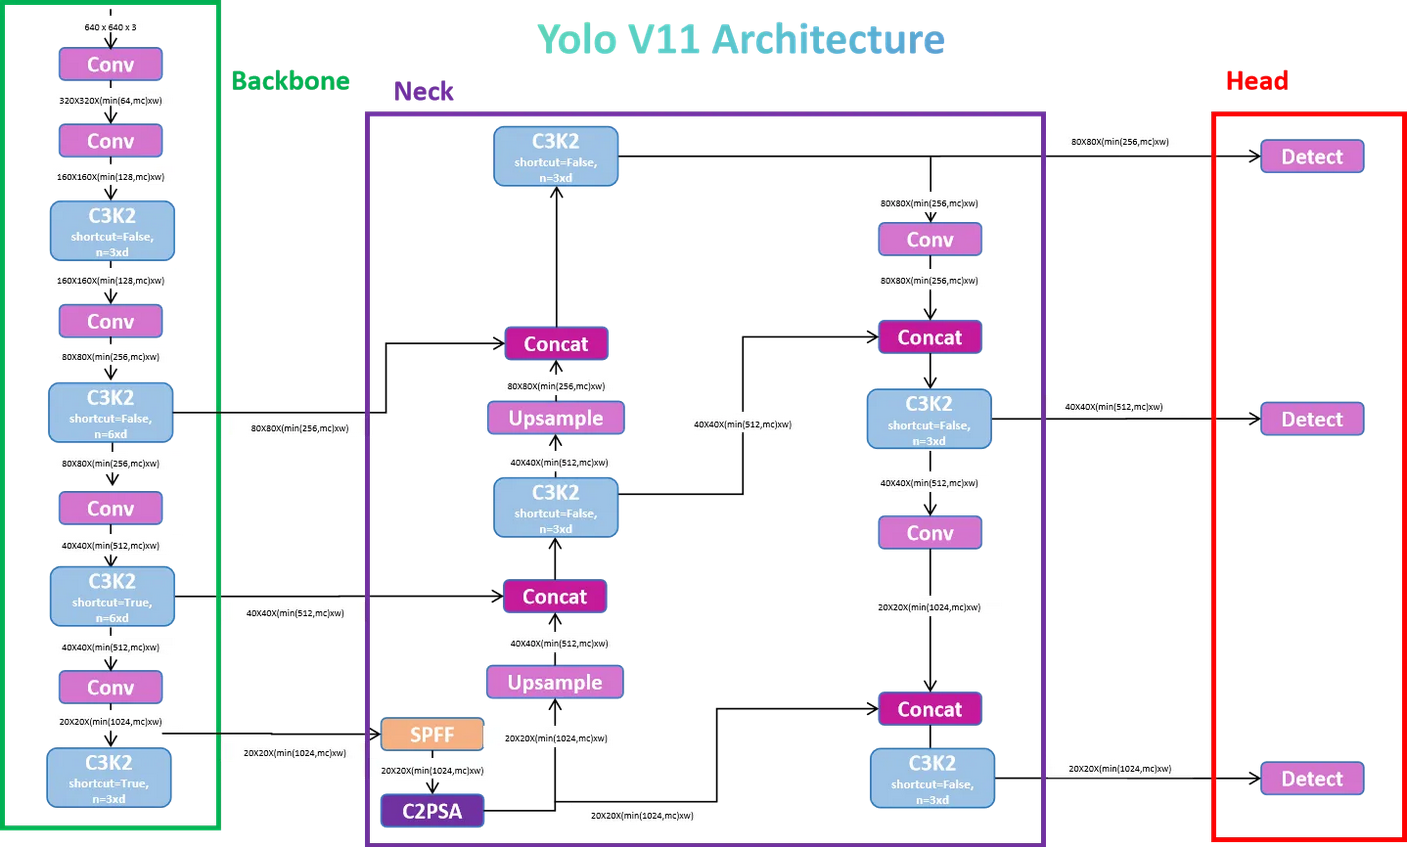
\includegraphics[width=0.85\textwidth]{YOLO_Architecture.png}
    \caption{Die Architektur von YOLOv11 \cite{Rao2024Oct}.}
    \label{fig:YOLO_Architecture}
\end{figure}

Im nächsten Schritt wurden die Einstellungen für die Datenaugmentation detailliert festgelegt. Dabei ist zu beachten, dass YOLO standardmäßig bereits mit vordefinierten Augmentationsmethoden arbeitet. Ein Teil des Projekts bestand jedoch darin, mit verschiedenen Augmentationsstrategien zu experimentieren und deren Einfluss auf die Modellleistung zu untersuchen. Eine detaillierte Darstellung des verwendeten Augmentation Codes und der jeweiligen Einstellungen in den verschiedenen Testfällen ist im Anhang dieses Dokuments zu finden.

Zusätzlich wurden die Trainingsparameter im Code definiert. Dazu gehörte unter anderem die Angabe des Trainingsdatensatzes sowie die Festlegung der Anzahl der Epochen. Eine Epoche beschreibt einen vollständigen Durchlauf durch den gesamten Trainings- und Validierungsdatensatz. Außerdem wurde die Art der verwendeten Datenaugmentierung spezifiziert. Eine Variante namens Strong Augmentation für starke Augmentation, eine Weak Augmentation für schwache Augmentation und eine No Augmentation für keine Augmentation. Dieser Codeabschnitt ist für das Training des Modells verantwortlich.

Nach Abschluss des Trainings wird automatisch ein Ordner mit dem Namen „runs/segment/train“ erzeugt. In diesem Ordner werden alle relevanten Informationen gespeichert. Dazu gehört auch der Unterordner „weights“, in dem sich die trainierten Gewichtungsdateien befinden. Insbesondere die Datei „best.pt“ stellt diejenige Version des Modells dar, die während des Trainings die besten Validierungsergebnisse erzielt hat. Dieses „best.pt“-Modell wird anschließend zur Evaluierung auf dem Testdatensatz verwendet. Dabei werden verschiedene Metriken, darunter mAP (mean Average Precision), Präzision und Recall, mithilfe eines einzigen YOLO-Befehls gemeinsam berechnet, um die Leistung des Modells objektiv zu bewerten.

Da die IoU (Intersection over Union) nicht standardmäßig als Einzelausgabe im Evaluierungsprozess von YOLO dargestellt wird, wurde im Rahmen dieses Projekts ein zusätzlicher Programmierabschnitt implementiert, um diese Kennzahl manuell zu berechnen. Dadurch wurde eine umfassendere Bewertung der Modellleistung ermöglicht. 

Zuletzt wurden außerdem der Segmentierungs-Loss und der Validierungs-Loss grafisch dargestellt.
Diese Visualisierungen sind entscheidend, um den Trainingsverlauf des Modells zu bewerten, insbesondere, um festzustellen, ob das Modell überfittet oder sich weiterhin stabil verbessert. Alle dabei erzeugten Metriken und Verlustwerte wurden gespeichert, um sie für eine spätere Analyse und zum Vergleich verschiedener Modelle nutzen zu können.

\section{Ergebnisse}
Mithilfe von YOLO wurden die Daten mit unterschiedlichen Einstellungen trainiert und die Ergebnisse anschließend miteinander verglichen. Zum Vergleich der Modelle wurden Metriken auf den Testdatensatz angewendet sowie der Segmentierungs-Loss für Training und Validierung bestimmt. 

Insgesamt wurden drei verschiedene Modelle verwendet. Ein vortrainiertes Modell von YOLO für die Segmentierung, ein nicht vortrainiertes Modell und ein vortrainiertes Modell für die medizinische Segmentierung. Das vortrainierte Modell für die medizinische Segmentierung ist speziell mit Ultraschallbildern von der Brust trainiert worden. Dabei ist dies 2023 veröffentlicht worden und verwendet YOLOv8. Somit ist dieses Modell speziell auf Ultraschallbilder trainiert worden und im Folgenden wird verglichen, ob dies einen Vorteil hat \cite{medical_imaging}.

Zunächst wurden alle drei Modellvarianten ohne Datenaugmentation miteinander verglichen.
Im Anschluss wurde das vortrainierte YOLOv11-Modell mit drei Augmentationsstrategien verglichen: ohne Augmentation, mit schwacher sowie mit starker Augmentation.
In einem weiteren Schritt wurde derselbe Vergleich für das nicht vortrainierte Modell durchgeführt, um die Auswirkungen unterschiedlicher Augmentationsstufen ohne Vortraining zu analysieren. Abschließend wurde das spezifisch für medizinische Segmentierungsaufgaben entwickelte, vortrainierte YOLO-Modell unter den gleichen Bedingungen evaluiert, um dessen Leistung im Vergleich zu den anderen Varianten einordnen zu können.

Was die Augmentationsstrategien betrifft, sind die Parameter für eine starke Augmentation verhältnismäßig hoch, für eine schwache niedriger und für keine Augmentation auf null eingestellt. Ein paar Parameter haben bei Graustufenbildern für die medizinische Segmentierung keinen oder nur einen geringen Einfluss. Dabei ist der hsv\_h für die Änderung des Farbtons zuständig und hsv\_s für die Sättigung. Bgr ändert die Reihenfolge der Farbkanäle und Mosaic kombiniert 4 Bilder zu einem großen Bild, was die anatomischen Zusammenhänge unnatürlich verändern kann. CutMix schneidet ein Rechteck aus einem Bild und fügt es in ein anderes ein. Dies kann die medizinischen Bilder zu stark verändern. MixUp mischt zwei Bilder und deren Labels. Dadurch werden die Bildinhalte vermischt und es sind unklare anatomische Strukturen vorhanden. Erasing legt ein schwarzes Rechteck zufällig über das Bild und könnte wichtige Bildmerkmale löschen. Die anderen Parameter sind entsprechend für schwache und starke Augmentation unterschiedlich hoch eingestellt. Dabei wurden für die starke Augmentation die Parameter nicht auf den höchstmöglichen Wert eingestellt, da der Datensatz nicht unnatürlich stark verändert werden sollte. In der Realität existieren solche Ultraschallaufnahmen nicht und es würde somit kein Modell für die realen Bedingungen erstellt werden. Die Einstellungen sind im Anhang zu finden.

\subsection{Trainings- und Validierungsverlust: Indikatoren für Overfitting}\label{sec:Trainings- und Validierungsverlust: Indikatoren für Overfitting}

Die Trainings- und Validierungsverluste sind in den Abbildungen~\ref{fig:no_aug},~\ref{fig:pretrainedv11},~\ref{fig:nopretrained} und~\ref{fig:pretrained_med} zu sehen. Auf der x-Achse ist die Anzahl der Epochen und auf der y-Achse der Segmentation-Loss-Wert aufgetragen. Dabei sind in blau die Trainings- und in orange die Validierungsverluste zu sehen.

Ein Vergleich der Modelle ohne Anwendung von Datenaugmentation ist in Abbildung~\ref{fig:no_aug} dargestellt. Das Verhalten des vortrainierten Modells, das speziell für medizinische Segmentierungsaufgaben entwickelt wurde, ist in Abbildung~\ref{fig:pretrained_med_no_aug} ersichtlich. Auffällig ist hierbei der deutliche Anstieg des Segmentierungsverlustes (Segmentation Loss) auf dem Validierungsdatensatz, während der Verlustwert auf den Trainingsdaten weiterhin sinkt. Dies wird als Overfitting bezeichnet und beschreibt die Situation, in der ein Modell die Trainingsdaten so stark „auswendig lernt“, dass es auf neuen, unbekannten Daten keine gute Leistung mehr zeigt \cite{dietterich1995overfitting}.

Der Segmentation Loss ist eine Metrik, die misst, wie stark die vom Modell vorhergesagten Segmentierungsmasken von den tatsächlichen Masken abweichen. Eine typische Loss-Funktion im Segmentierungskontext ist zum Beispiel der Dice Loss \cite{Ultralytics2025Jul}.

Ein gut generalisierendes Modell sollte einen möglichst niedrigen Segmentierungsverlust sowohl auf den Trainings- als auch auf den Validierungsdaten aufweisen, und dabei über mehrere Epochen hinweg gleichmäßig lernen. Ein stabiler Verlauf deutet darauf hin, dass das Modell sowohl die Struktur der Daten erlernt als auch in der Lage ist, dieses Wissen auf bisher ungesehene Daten zu übertragen.

Die Abbildungen~\ref{fig:Nopretrainedv11_no_aug_10} und~\ref{fig:pretrainedv11_no_aug} zeigen Trainingsverläufe von Modellen, die ebenfalls ohne Datenaugmentation trainiert wurden. Die Lernkurven dieser Modelle sind flacher und zeigen eine längere Trainingsdauer, jedoch bleiben die Werte des Segmentierungsverlustes insgesamt hoch. Dies weist auf ein geringes Leistungsniveau hin, möglicherweise aufgrund der geringen Datenmenge oder fehlender regulierender Maßnahmen wie Augmentation.

\begin{figure}[h]
    \centering
    \begin{subfigure}[b]{0.3\textwidth}
        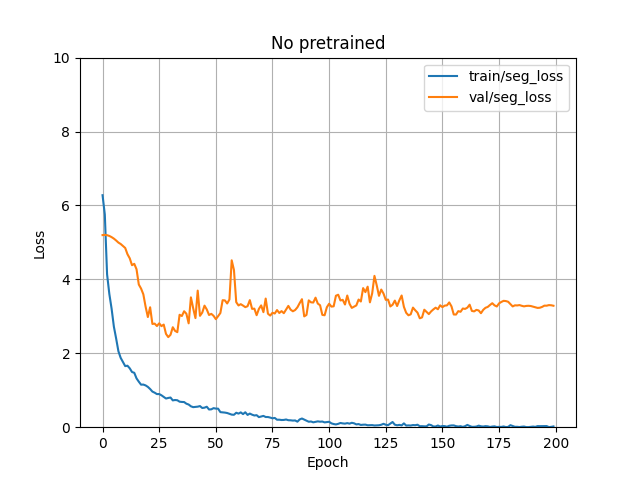
\includegraphics[width=\textwidth]{Nopretrainedv11_no_aug_10}
        \caption{Nicht vor trainiertes Modell.}
        \label{fig:Nopretrainedv11_no_aug_10}
    \end{subfigure}
    \hfill
    \begin{subfigure}[b]{0.3\textwidth}
        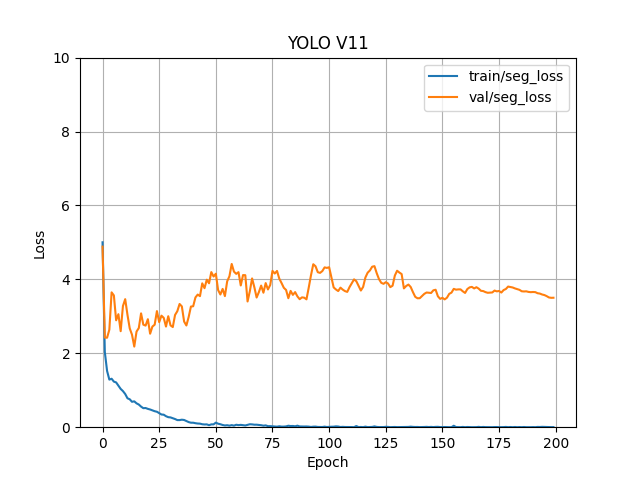
\includegraphics[width=\textwidth]{pretrainedv11_no_aug}
        \caption{Vortrainiertes YOLOv11-Modell für die Segmentation.}
        \label{fig:pretrainedv11_no_aug}
    \end{subfigure}
    \hfill
    \begin{subfigure}[b]{0.3\textwidth}
        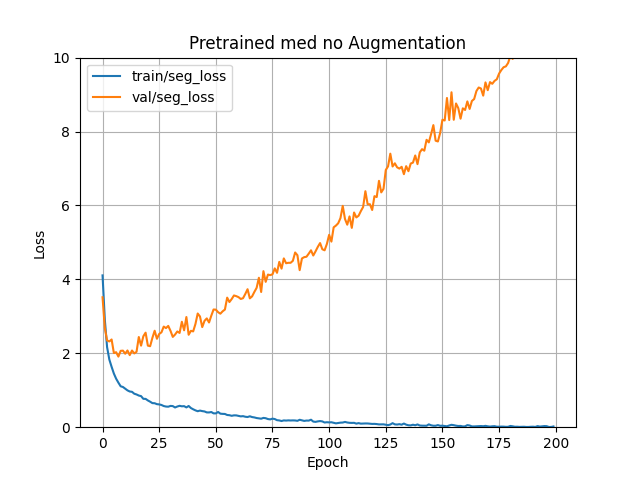
\includegraphics[width=\textwidth]{pretrained_med_no_aug}
        \caption{Vortrainiertes Modell für die medizinische Segmentation.}
        \label{fig:pretrained_med_no_aug}
    \end{subfigure}    
    \caption{Vergleich unterschiedlicher vortrainierter und nicht vortrainierter Modelle.}
    \label{fig:no_aug}
\end{figure}

Eine gezielte Datenaugmentation kann helfen, Overfitting zu reduzieren und die Generalisierung des Modells zu verbessern.

In Abbildung~\ref{fig:pretrainedv11} sind die Verläufe des vortrainierten YOLOv11-Modells mit unterschiedlichen Augmentationsparametern dargestellt. Es zeigt sich deutlich, dass der Einsatz von Datenaugmentation zu einem insgesamt niedrigeren Segmentation Loss führt, wie in Abbildung~\ref{fig:pretrainedv11_weak_aug} (schwache Augmentation) und Abbildung~\ref{fig:pretrainedv11_strong_aug} (starke Augmentation) ersichtlich ist. Die Abbildung~\ref{fig:pretrainedv11_strong_aug} zeigt das Modell mit der starken Augmentation und sieht im Vergleich zu den anderen Modellen am besten aus. Der Segmentation Loss sinkt kontinuierlich über einen längeren Trainingszeitraum, was auf eine verbesserte Generalisierungsfähigkeit hindeutet. Dies lässt darauf schließen, dass in diesem Fall eine gezielt eingesetzte, stärkere Datenaugmentation zur Vermeidung von Overfitting beiträgt und die Leistungsfähigkeit des Modells auf bisher ungesehene Daten verbessert. 

\begin{figure}[H]
    \centering
    \begin{subfigure}[b]{0.3\textwidth}
        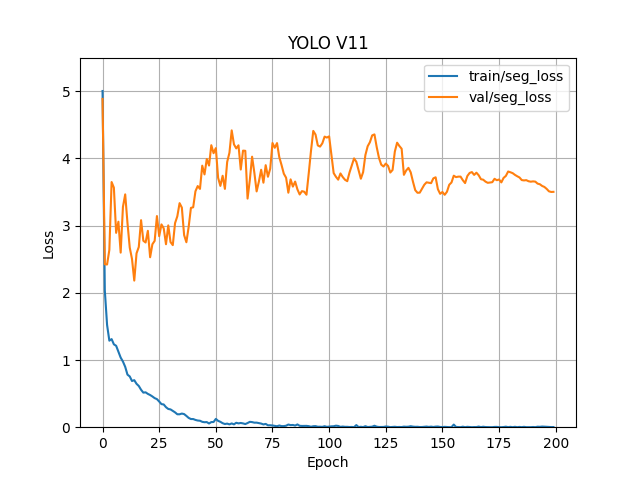
\includegraphics[width=\textwidth]{pretrainedv11_no_aug_5.5}
        \caption{Vortrainiertes Modell von YOLOv11 für die Segmentation.}
        \label{fig:pretrainedv11_no_aug_5.5}
    \end{subfigure}
    \hfill
    \begin{subfigure}[b]{0.3\textwidth}
        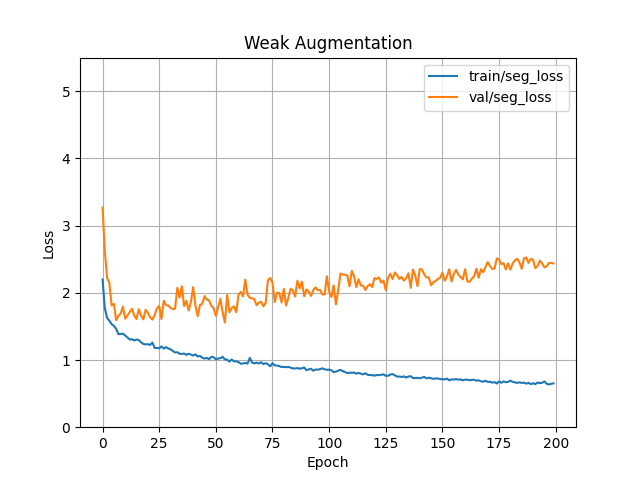
\includegraphics[width=\textwidth]{pretrainedv11_weak_aug}
        \caption{Vortrainiertes Modell von YOLOv11 für die Segmentation mit schwacher Augmentation.}
        \label{fig:pretrainedv11_weak_aug}
    \end{subfigure}
    \hfill
    \begin{subfigure}[b]{0.3\textwidth}
        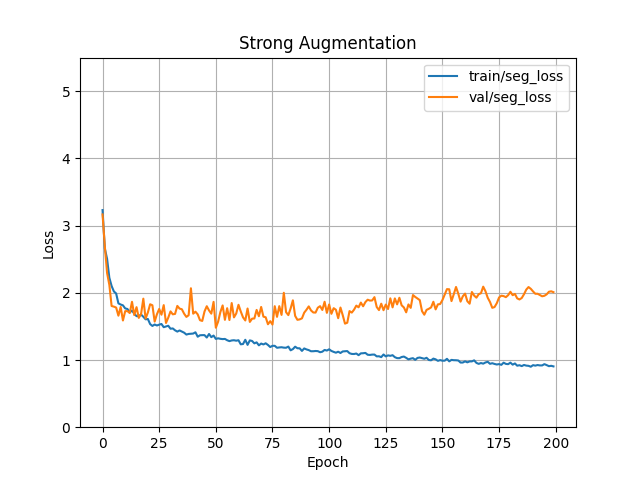
\includegraphics[width=\textwidth]{pretrainedv11_strong_aug}
        \caption{Vortrainiertes Modell von YOLOv11 für die Segmentation mit starker Augmentation.}
        \label{fig:pretrainedv11_strong_aug}
    \end{subfigure}    
    \caption{Vergleich des vortrainierten YOLOv11-Modells für die Segmentation mit unterschiedlichen Augmentierungsparametern.}
    \label{fig:pretrainedv11}
\end{figure}

Ein weiterer Vergleich der Trainingsverläufe ist in Abbildung~\ref{fig:nopretrained} dargestellt, in der ein nicht vortrainiertes YOLOv11-Modell mit und ohne Datenaugmentation untersucht wird. Analog zu den zuvor beschriebenen Ergebnissen zeigt sich auch hier, dass der Einsatz von Augmentation einen positiven Einfluss auf das Trainingsverhalten hat. Insbesondere das Modell mit starker Augmentation weist einen länger andauernden Trainingsprozess auf, erkennbar an dem verzögerten Anstieg des Validierungsverlusts. Gleichzeitig ist der Segmentation Loss im Vergleich zur Variante ohne Augmentation deutlich reduziert. Dies deutet darauf hin, dass auch bei nicht vortrainierten Modellen eine geeignete Augmentationsstrategie die Generalisierungsfähigkeit verbessert und dem frühzeitigen Overfitting entgegenwirkt.

\begin{figure}[H]
    \centering
    \begin{subfigure}[b]{0.3\textwidth}
        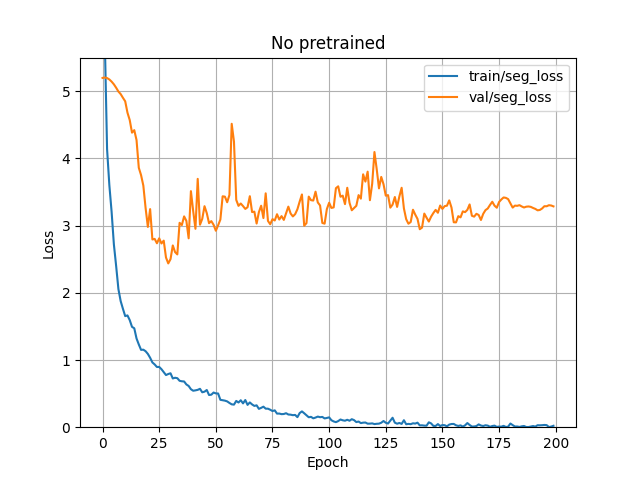
\includegraphics[width=\textwidth]{Nopretrainedv11_no_aug.png}
        \caption{Nicht vortrainiertes Modell ohne Augmentation.}
        \label{fig:nopretrainedv11_no_aug}
    \end{subfigure}
    \hfill
    \begin{subfigure}[b]{0.3\textwidth}
        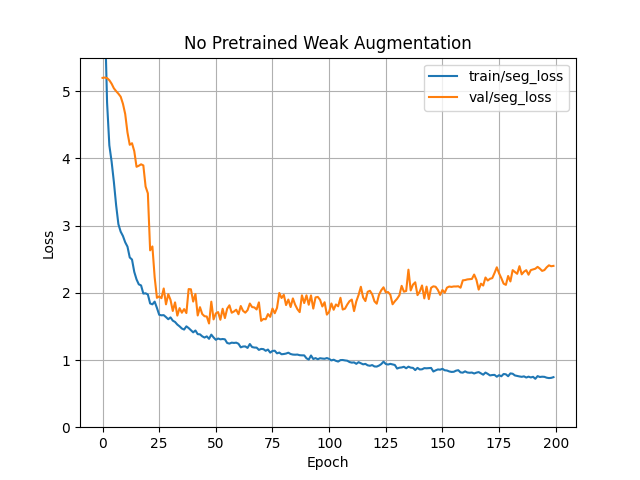
\includegraphics[width=\textwidth]{nopretrained_weak_aug}
        \caption{Nicht vortrainiertes Modell mit schwacher Augmentation.}
        \label{fig:nopretrained_weak_aug}
    \end{subfigure}
    \hfill
    \begin{subfigure}[b]{0.3\textwidth}
        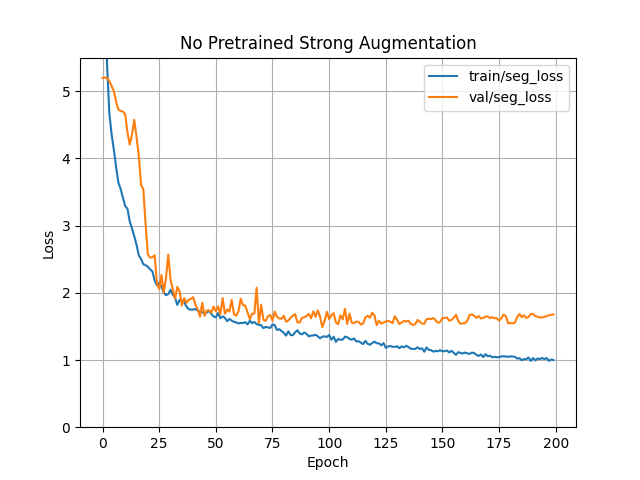
\includegraphics[width=\textwidth]{nopretrained_strong_aug}
        \caption{Nicht vortrainiertes Modell mit starker Augmentation}
        \label{fig:nopretrained_strong_aug}
    \end{subfigure}    
    \caption{Vergleich des nicht vortrainierten Modells mit unterschiedlichen Augmentierungsparametern.}
    \label{fig:nopretrained}
\end{figure}

Zuletzt ist in Abbildung~\ref{fig:pretrained_med} der Vergleich zwischen dem vortrainierten medizinischen Modell ohne, mit starker und schwacher Augmentation zu sehen. Hier ist wieder der positive Einfluss von Augmentation in den Abbildungen~\ref{fig:pretrained_med_weak_aug} und \ref{fig:pretrained_med_strong_aug} zu sehen. Dies zeigt erneut den Nutzen geeigneter Augmentationsverfahren zur Verbesserung der Modellgeneralisation, selbst bei bereits spezialisierten, vortrainierten Architekturen.

\begin{figure}[H]
    \centering
    \begin{subfigure}[b]{0.3\textwidth}
        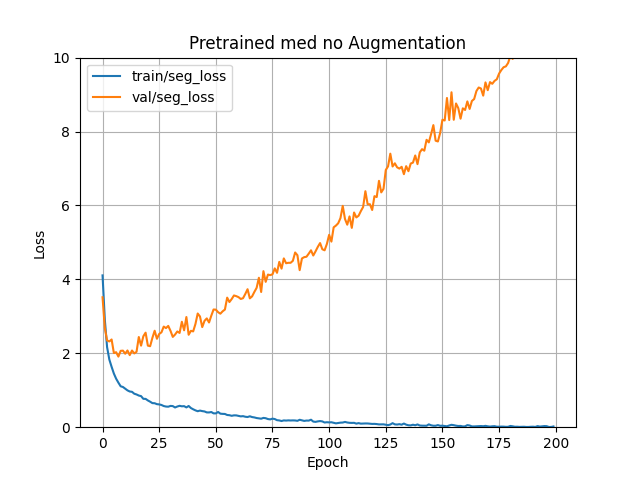
\includegraphics[width=\textwidth]{pretrained_med_no_aug.png}
        \caption{Vortrainiertes medizinisches Segmentierungsmodell.}
        \label{fig:pretrained_med_no_aug2}
    \end{subfigure}
    \hfill
    \begin{subfigure}[b]{0.3\textwidth}
        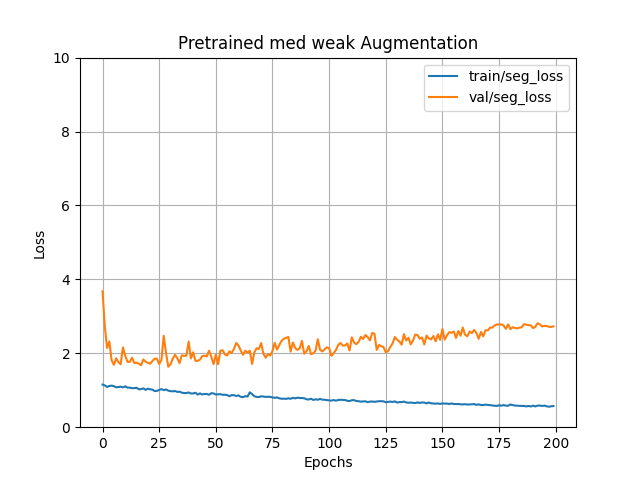
\includegraphics[width=\textwidth]{pretrained_med_weak_aug.png}
        \caption{Vortrainiertes medizinisches Segmentierungsmodell mit schwacher Augmentation.}
        \label{fig:pretrained_med_weak_aug}
    \end{subfigure}
    \hfill
    \begin{subfigure}[b]{0.3\textwidth}
        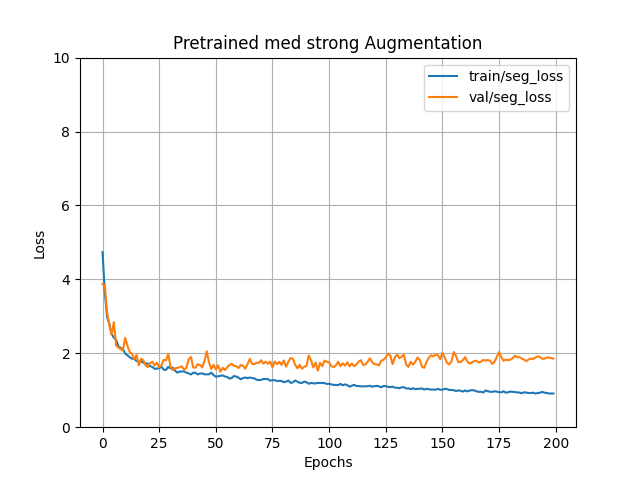
\includegraphics[width=\textwidth]{pretrained_med_strong_aug.png}
        \caption{Vortrainiertes medizinisches Segmentierungsmodell mit starker Augmentation.}
        \label{fig:pretrained_med_strong_aug}
    \end{subfigure}    
    \caption{Vergleich des vortrainierten medizinischen Modells mit unterschiedlichen Augmentierungsparametern.}
    \label{fig:pretrained_med}
\end{figure}


\subsection{Auswertung anhand von Metriken}
Die Ergebnisse der Auswertung anhand der Metriken und des Testdatensatzes sind in den Tabellen~\ref{tab:modelle-metriken}, \ref{tab:yolov11-augmentation} und \ref{tab:yolov11-no-pretrain} dargestellt. Dabei wurden die Modelle mit den Metriken „Intersection over Union” (IoU), „Präzision” (P), „Recall” (R) und „mAP50” bewertet.

Zunächst werden in Tabelle~\ref{tab:modelle-metriken} die drei Modellvarianten ohne Augmentation miteinander verglichen. Das YOLOv11-Modell zeigt mit einem IoU-Wert von 0.412 und einem mAP50 von 0.429 die beste Leistung im Vergleich, insbesondere auch im Recall mit 0.619. Das medizinisch vortrainierte Modell weist hingegen eine höhere Präzision (0.401) auf.

\begin{table}[H]
\centering
\begin{tabular}{l|c|c|c}
\textbf{} & \textbf{Vortrainiertes YOLOv11-Modell} & \textbf{Nicht vortrainiertes Modell} & \textbf{Vortrainiertes Modell med.Segmentation} \\
\hline
IoU     & \textbf{0.412} & 0.322 & 0.406 \\
P       & 0.373 & 0.226 & \textbf{0.401} \\
R       & \textbf{0.619} & 0.290 & 0.416 \\
mAP50   & \textbf{0.429} & 0.244 & 0.376 \\
\end{tabular}
\caption{Vergleich unterschiedlicher vortrainierter und nicht vortrainierter Modelle.}
\label{tab:modelle-metriken}
\end{table}

In Tabelle ~\ref{tab:yolov11-augmentation} werden anschließend die Ergebnisse des vortrainierten YOLOv11-Modells unter verschiedenen Augmentationsstrategien analysiert. Es zeigt sich, dass die schwache Augmentation zu den besten Ergebnissen führt: Sie erreicht einen IoU von 0.653, einen mAP50 von 0.448 und den höchsten Recall-Wert (0.652). Dies lässt den Schluss zu, dass eine moderate Datenaugmentation die Lernfähigkeit des Modells verbessern kann, ohne die Bildinformationen zu stark zu verändern.

\begin{table}[H]
\centering
\begin{tabular}{l|c|c|c}
\textbf{} & \textbf{No Augmentation} & \textbf{Schwache Augmentation} & \textbf{Starke Augmentation} \\
\hline
IoU     & 0.411 & \textbf{0.653} & 0.627 \\
P       & 0.373 & \textbf{0.425} & 0.423 \\
R       & 0.619 & \textbf{0.652} & 0.542 \\
mAP50   & 0.429 & \textbf{0.448} & 0.372 \\
\end{tabular}
\caption{Vergleich des vortrainierten YOLOv11-Modells für die Segmentation mit unterschiedlichen Augmentierungsparametern.}
\label{tab:yolov11-augmentation}
\end{table}

Die Tabelle ~\ref{tab:yolov11-no-pretrain} enthält die Auswertung des nicht vortrainierten Modells unter den gleichen Augmentationsbedingungen. Interessanterweise erzielt dieses Modell die besten Ergebnisse bei starker Augmentation: Es erreicht einen IoU von 0.662, einen mAP50 von 0.507 und eine deutlich höhere Präzision (0.534) als bei den anderen Augmentationsstufen. Daraus lässt sich schließen, dass eine stärkere Datenvariation bei Modellen ohne Vortraining hilfreich sein kann, um die Generalisierungsfähigkeit zu erhöhen.

\begin{table}[H]
\centering
\begin{tabular}{l|c|c|c}
\textbf{} & \textbf{No Augmentation} & \textbf{Schwache Augmentation} & \textbf{Starke Augmentation} \\
\hline
IoU     & 0.325 & 0.622 & \textbf{0.662} \\
P       & 0.226 & 0.298 & \textbf{0.534} \\
R       & 0.291 & 0.464 & \textbf{0.531} \\
mAP50   & 0.244 & 0.299 & \textbf{0.507} \\
\end{tabular}
\caption{Vergleich des nicht vortrainierten Modells mit unterschiedlichen Augmentierungsparametern.}
\label{tab:yolov11-no-pretrain}
\end{table}

Schließlich wurde das vortrainierte Modell für die medizinische Segmentierung ebenfalls mit verschiedenen Augmentationsparametern getestet. Die Ergebnisse dieser Auswertung sind in Tabelle ~\ref{tab:pretrained-med-aug} dargestellt. Die Metriken zeigen, dass sowohl die schwache als auch die starke Augmentation zu einer deutlichen Leistungssteigerung im Vergleich zum Modell ohne Augmentation führen. Besonders auffällig ist der Anstieg des IoU-Wertes von 0.406 (ohne Augmentation) auf 0.622 bei beiden Augmentationsstrategien. Auch die Precision verbessert sich von 0.401 auf 0.427 bei schwacher und auf 0.455 bei starker Augmentation. Die Recall-Werte steigen ebenfalls erheblich: von 0.416 auf 0.695 (schwach) bzw. 0.652 (stark). Der mAP50-Wert erreicht mit starker Augmentation den Höchstwert von 0.495.

Diese Ergebnisse zeigen, dass die Wahl geeigneter Augmentationsmethoden auch bei einem fachspezifisch vortrainierten Modell einen erheblichen Einfluss auf die Modellleistung hat.
\begin{table}[H]
\centering
\begin{tabular}{l|c|c|c}
& \textbf{No Augmentation} & \textbf{Schwache Augmentation} & \textbf{Starke Augmentation} \\
\hline
IoU & 0.406 & \textbf{0.622} & \textbf{0.622} \\
P & 0.401 & 0.427 & \textbf{0.455} \\
R & 0.416 & \textbf{0.695} & 0.652 \\
mAP50 & 0.376 & 0.477 & \textbf{0.495} \\
\end{tabular}
\caption{Vergleich des vortrainierten medizinischen Modells mit unterschiedlichen Augmentationsparametern.}
\label{tab:pretrained-med-aug}
\end{table}

\section{Diskussion und Fazit}
Ziel dieser Arbeit war es, die automatische Segmentierung submentaler Muskeln und deren Morphologie in Ultraschallbildern mittels eines YOLOv11-basierten Deep-Learning-Ansatzes zu untersuchen.

Bei der Analyse der Trainings- und Validierungsverluste, wie in Abschnitt~\ref{sec:Trainings- und Validierungsverlust: Indikatoren für Overfitting} beschrieben, zeigt sich, dass bei dem kleinen Datensatz von 300 Bildern die Datenaugmentation das Ergebnis verbessert. Das nicht vortrainierte YOLOv11-Modell mit starker Augmentation (vgl. Abbildung~\ref{fig:nopretrained_strong_aug}) erscheint dort am besten. Der Segmentation Loss sinkt über einen längeren Trainingszeitraum, was auf eine verbesserte Generalisierungsfähigkeit hindeutet, im Vergleich zu den anderen Modellen. Ein möglicher Grund dafür ist, dass die vortrainierten Modelle nicht spezifisch auf die Segmentierung von Muskelstrukturen in Ultraschallbildern optimiert wurden. Insbesondere das medizinisch vortrainierte Modell wurde zwar auf Ultraschallbildern trainiert, jedoch mit einem anders fokussierten Zielbereich.

Bei der Auswertung der auf den Testdatensatz angewendeten Metriken zeigt sich, dass Modelle mit Datenaugmentation tendenziell bessere Ergebnisse erzielen, was unter anderem auf die geringe Größe des Datensatzes zurückzuführen ist. Die Ausprägung des Effekts hängt jedoch davon ab, ob das Modell vortrainiert ist oder nicht. Eine schwache Augmentation verändert den Datensatz nur geringfügig. Bei vortrainierten Modellen mit schwacher Augmentation kann so stärker auf das bereits erworbene Wissen aus dem Pretraining zurückgegriffen werden. Im Gegensatz dazu verändert eine starke Augmentation den Datensatz deutlicher, wodurch der Einfluss der vortrainierten Gewichte reduziert wird. Bei vortrainierten Modellen wird ein nicht so großer Datensatz benötigt, da diese auf eine spezifische Aufgabe spezialisiert sind. Dies erklärt, warum bei den Metriken vortrainierte Modelle mit schwacher Augmentation tendenziell besser abschneiden. Für nicht vortrainierte Modelle hingegen erweist sich eine starke Augmentation als vorteilhaft. Da diese Modelle von Grund auf trainiert werden müssen, ist das Risiko von Overfitting bei kleinen Datensätzen höher. Durch die starke Augmentation wird die Vielfalt der Trainingsdaten erhöht, was zu einem längeren und stabileren Lernprozess führt. 

Die Unterschiede zwischen einigen Modellen fielen jedoch relativ gering aus, was unter anderem auf die begrenzte Anzahl an Testdaten zurückgeführt werden kann. Die Ergebnisse in Abbildung~\ref{fig:Testdaten} illustrieren die Segmentierungsergebnisse des nicht vortrainierten Modells mit starker Augmentation. Hier zeigte sich, dass teilweise vier statt drei Regionen erkannt wurden. Dies sollte in zukünftigen Arbeiten weiter optimiert werden.

\begin{figure}[H]
    \centering
    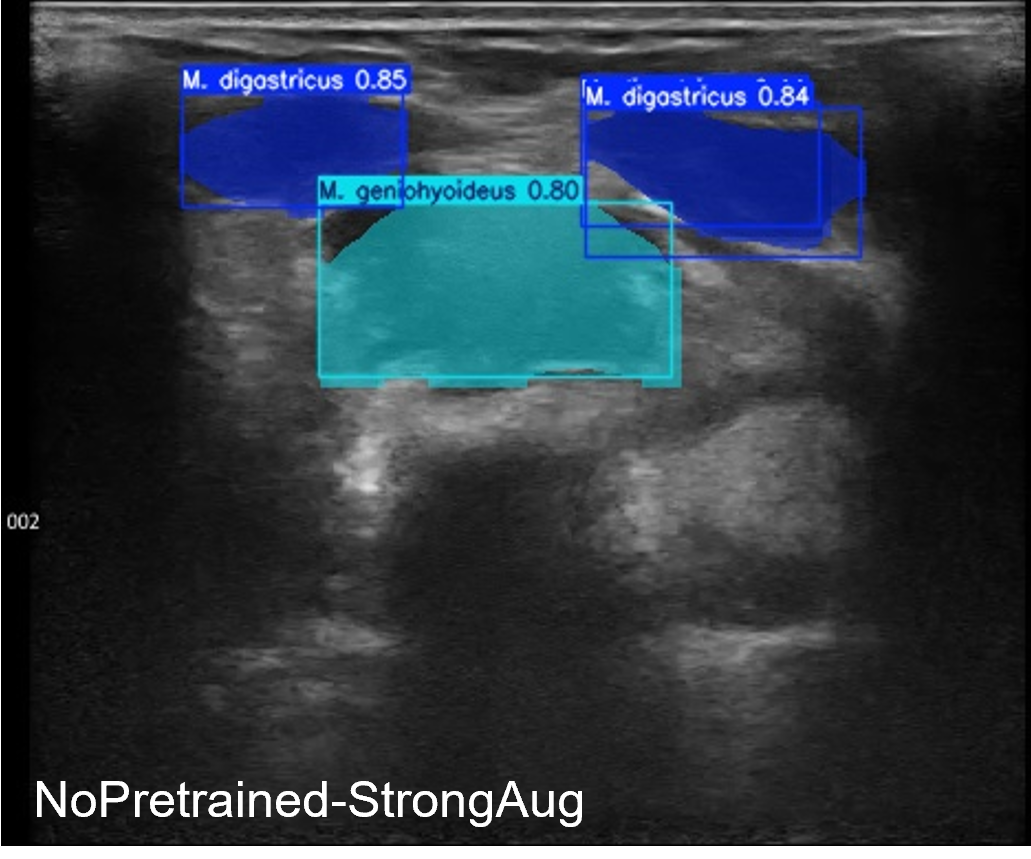
\includegraphics[width=0.5\textwidth]{no_pretrained_stronAug_testbild.png}
    \caption{Hier wurde das nicht vortrainierte Modell mit starker Augmentation auf ein Bild im Testdatensatz angewendet.}
    \label{fig:Testdaten}
\end{figure}

Für weitere Arbeiten, wäre es sinnvoll mehr Ultraschallbilder von weiteren Probanden zu segmentieren. Von Interesse wäre es, die Vielfalt der Probanden zu erhöhen. Es könnte zum Beispiel die Altersspanne erhöht werden und ebenfalls kranke Probanden betrachtet werden. Dadurch kann die Generalisierbarkeit und Robustheit des Modells verbessert werden. Des Weiteren könnte der Einfluss verschiedener Schlucksubstanzen auf die Muskelmorphologie analysiert werden. Es könnte dort mithilfe der Segmentierung die Form und Größe des Muskels weiter untersucht werden. Mit den Videoaufnahmen könnte auch der Schluckvorgang in Abhängigkeit der Zeit untersucht werden. 

In Zukunft könnte durch weitere Studien eine KI-gestützte Metrik zur Identifikation von Schluckstörungen (Dysphagie) entwickelt und standardisiert werden. 
Dazu bedarf es jedoch weiterer klinischer Validierungen und einer Standardisierung der Segmentierungsmethodik im medizinischen Kontext.
\newpage
\section{Anhang}
\subsection{Code}
\begin{minted}[fontsize=\small, breaklines]{python}

# Installieren der ultralytics Bibliothek
pip install ultralytics

# Ein vortrainiertes Model für YOLOv8 für medizinische Segmentierung
wget https://github.com/sevdaimany/YOLOv8-Medical-Imaging/raw/master/runs/segment/train/weights/best.pt -O yolov8n-medicalImaging.pt

# Importieren von YOLO
from ultralytics import YOLO

#Laden eines Modells und der Rest rauskommentiert
model = YOLO('yolo11n-seg.pt') # load a pretrained model 
model = YOLO("yolov8n-medicalImaging.pt") # load a pretrained medical imaging model
model = YOLO("yolo11n-seg.yaml")  # build a new model from YAML

#Einstellen des Augmentations
strong_aug = {
    "dropout": 0.4, #Dropout rate for regularization in classification tasks, preventing overfitting by randomly omitting units during training.
    "hsv_h": 0, #Adjusts the hue of the image
    "hsv_s": 0, #Alters the saturation of the image
    "hsv_v": 0.5, # Modifies the value (brightness) of the image
    "degrees": 30.0, # 30 Rotates the image randomly within the specified degree range
    "translate": 0.1, #Translates the image horizontally and vertically by a fraction of the image size
    "scale": 0.3, #Scales the image by a gain factor
    "shear": 5, #Shears the image by a specified degree
    "perspective": 0.0001, #Applies a random perspective transformation to the image
    "flipud": 0.5, #Flips the image upside down with the specified probability
    "fliplr": 0.7, #Flips the image left to right with the specified probability
    "bgr": 0, #Flips the image channels from RGB to BGR
    "mosaic": 0, #Combines four training images into one, simulating different scene compositions and object interactions. Highly effective for complex scene understanding.
    "mixup": 0, #Blends two images and their labels, creating a composite image. Enhances the model's ability to generalize by introducing label noise and visual variability.
    "cutmix": 0, #Combines portions of two images, creating a partial blend while maintaining distinct regions. Enhances model robustness by creating occlusion scenarios.
    "erasing": 0, #Classification only. Randomly erases regions of the image during training to encourage the model to focus on less obvious features.
}

no_aug = {
    "dropout": 0,
    "hsv_h": 0,
    "hsv_s": 0,
    "hsv_v": 0,
    "degrees": 0.0,
    "translate": 0.0,
    "scale": 0.0,
    "shear": 0,
    "perspective": 0,
    "flipud": 0.0,
    "fliplr": 0.0,
    "bgr": 0,
    "mosaic": 0,
    "mixup": 0,
    "cutmix": 0,
    "erasing": 0,
}

weak_aug = {
    "dropout": 0.2,
    "hsv_h": 0,
    "hsv_s": 0,
    "hsv_v": 0.1,
    "degrees": 10.0,
    "translate": 0.05,
    "scale": 0.3,
    "shear": 0,
    "perspective": 0,
    "flipud": 0,
    "fliplr": 0.5,
    "bgr": 0,
    "mosaic": 0,
    "mixup": 0,
    "cutmix": 0,
    "erasing": 0,
}

#Einstellung von Trainingsparametern und trainieren des Modells mit dem Dataset
model.train(
    data='/content/drive/MyDrive/dataset/data.yaml',
    epochs=200,
    imgsz=640,
    #amp=False,
    #lr0=0.0005,
    overlap_mask=False,
    mask_ratio=1,
    batch=32,
    patience=200,
    #freeze=23,
    **strong_aug #Gewünschte Augmentation eingeben
    )

#Berechnen IoU
import os
import cv2
import numpy as np
from tqdm import tqdm

model = YOLO("/content/runs/segment/train/weights/best.pt")
# Paths to test images and labels
img_dir = "/content/drive/MyDrive/dataset/test/images/test"
label_dir = "/content/drive/MyDrive/dataset/test/labels/test"

# Helper: Convert YOLO polygon annotation to a binary mask
def polygon_to_mask(img_shape, polygon):
    mask = np.zeros(img_shape, dtype=np.uint8)
    pts = np.array(polygon, np.int32).reshape((-1, 2))
    cv2.fillPoly(mask, [pts], 1)
    return mask

# Store IoUs
ious = []

# Iterate over all test images
for img_file in tqdm(os.listdir(img_dir)):
    if not img_file.endswith((".jpg", ".png", ".jpeg")):
        continue

    # Load image
    img_path = os.path.join(img_dir, img_file)
    image = cv2.imread(img_path)
    h, w = image.shape[:2]

    # Predict with model (resizes to 512 by default)
    results = model.predict(img_path, conf=0.25, save=False)[0]
    pred_masks = results.masks.data.cpu().numpy() if results.masks else []

    # Load ground truth polygons
    label_file = img_file.rsplit(".", 1)[0] + ".txt"
    label_path = os.path.join(label_dir, label_file)
    if not os.path.exists(label_path):
        continue

    with open(label_path, "r") as f:
        lines = f.readlines()

    for line in lines:
        parts = line.strip().split()
        if len(parts) <= 5:
            continue  # skip if no polygon

        polygon = list(map(float, parts[5:]))
        polygon[::2] = [x * w for x in polygon[::2]]  # scale x
        polygon[1::2] = [y * h for y in polygon[1::2]]  # scale y

        gt_mask = polygon_to_mask((h, w), polygon)

        # Match with best predicted mask (resized to original shape)
        best_iou = 0
        for pm in pred_masks:
            pred_mask = (pm > 0.5).astype(np.uint8)
            pred_mask_resized = cv2.resize(pred_mask, (w, h), interpolation=cv2.INTER_NEAREST)

            intersection = np.logical_and(gt_mask, pred_mask_resized).sum()
            union = np.logical_or(gt_mask, pred_mask_resized).sum()
            if union > 0:
                iou = intersection / union
                best_iou = max(best_iou, iou)

        ious.append(best_iou)

# Compute mean IoU
if ious:
    mean_iou = np.mean(ious)
    print(f"Mean IoU over {len(ious)} masks: {mean_iou:.4f}")
else:
    print("No IoUs could be calculated — check label/prediction format.")


#Berechnen der Metriken mit dem Testdatensatz
yolo task=segment mode=val model=/content/ runs/segment/train/weights/best.pt 
data=/content/drive/MyDrive/dataset/data_test.yaml split=test

# Plotten der train/seg_loss und val/seg_loss werten
import pandas as pd
import matplotlib.pyplot as plt
# Pfad der Datei
path = "/content/ runs/segment/train/results.csv"
path_run = "/content/runs/segment/train/results.csv"
df = pd.read_csv(path)
# Definieren der x-/y-Achse
df = df[["train/seg_loss", "val/seg_loss"]]
df.plot(ylim=(0, 5.5), grid=True)
plt.xlabel("Epoch")
plt.ylabel("Loss")
# Titel des Plots
plt.title("No Pretrained Strong Augmentation")
# Speichern des Plots
plt.savefig('nopretrained_strong_aug.png')

#Model auf Bilder laufen lassen
yolo predict model=/content/runs/segment/train/weights/best.pt  source=/content/drive/MyDrive/US_Projekt/frames line_width=1 conf=0.1 

#Model auf video laufen lassen
yolo predict model=/content/runs/segment/train/weights/best.pt source=/content/drive/MyDrive/US_Projekt/frames/Video_probe line_width=1 conf=0.1 #Path achten
ffmpeg -i runs/segment/predict2/0.avi -vcodec libx264 -crf 23 -preset medium output.mp4
\end{minted}
\newpage
\printbibliography

\end{document}

\newpage
\begin{thebibliography}{99}
\bibitem{ref1} World Gastroenterology Organisation. \textit{Dysphagia – Global Guidelines}. Available at: \url{https://www.worldgastroenterology.org/guidelines/dysphagia} (besucht am 28.07.2025). 
\bibitem{ref2} M. Hsiao, Y. Chang, W. Chen, H. Chang, T. Wang, \textit{Application of Ultrasonography in Assessing Oropharyngeal Dysphagia in Stroke Patients}. Ultrasound in Medicine and Biology, Jg.38, Nr.9, S.1522-1528, 2012. doi:\url{https://doi.org/10.1016/j.ultrasmedbio.2012.04.017                                                                           }.
\bibitem{ref3} K. Barron, M. Blaivas, L. Blaivas, J. Sadler, I. Deal, \textit{Bedside Ultrasound to Identify and Predict Severity of Dysphagia Following Ischemic Stroke: Human Versus Artificial Intelligence}. Ultrasound in Medicine and Biology, Jg.50, Nr.1, S.99-104, 2024. doi:\url{https://doi.org/10.1016/j.ultrasmedbio.2023.09.008                                                                         }.
\bibitem{ref4} C. Chakraborty, M. Bhattacharya, S. Pal, S. Lee \textit{From machine learning to deep learning: Advances of the recent data-driven paradigm shift in medicine and healthcare}. Current Research in Biotechnology, Nr.7, S.100164, 2024. doi:\url{https://doi.org/10.1016/j.crbiot.2023.100164                                                                         }.
\bibitem{ref5} B. Zhou, X. Yang, W. Curran, T. Liu, \textit{Artificial Intelligence in Quantitative Ultrasound Imaging: A Survey}. 
Journal of Ultrasound in Medicine, Jg.41, Nr.6, S.1329-1342, 2022. Doi:\url{https://doi.org/10.1002/jum.15819                                                                }

\end{thebibliography}